%!TEX TS-program = pdflatex
% dissertation.tex -- main dissertation file
%
% Wisconsin dissertation template
% Copyright (c) 2008-2009 William C. Benton.  All rights reserved.
%
% This program can redistributed and/or modified under the terms
% of the LaTeX Project Public License Distributed from CTAN
% archives in directory macros/latex/base/lppl.txt; either
% version 1 of the License, or (at your option) any later version.
%
% This program includes other software that is licensed under the
% terms of the LPPL and the Perl Artistic License; see README for details.
%
% You, the user, still hold the copyright to any document you produce
% with this software (like your dissertation).
%

%%% You'll want ``oneside'' for the deposit version, but probably not for any versions that don't need to meet the UW requirements
\documentclass[12pt,oneside,letterpaper]{memoir}

% preamble.tex -- packages to include
%
% Wisconsin dissertation template
% Copyright (c) 2008 William C. Benton.  All rights reserved.
%
% This program can redistributed and/or modified under the terms
% of the LaTeX Project Public License Distributed from CTAN
% archives in directory macros/latex/base/lppl.txt; either
% version 1 of the License, or (at your option) any later version.
%
% This program includes other software that is licensed under the
% terms of the LPPL and the Perl Artistic License; see README for details.
%
% You, the user, still hold the copyright to any document you produce
% with this software (like your dissertation).

%% You should use natbib
\IfFileExists{natbib.sty}{%
\usepackage[numbers,sort]{natbib}%
}{}

%% You probably need appendix, if you want appendices
\IfFileExists{appendix.sty}{%
\usepackage{appendix}%
}{}

%% the spacing in memoir is weird, you'll need to use this
\DisemulatePackage{setspace}
\usepackage[onehalfspacing]{setspace}

%% List setup; the ``hanglist`` environment will allow you to have
%% nicely-typeset enumerated lists (i.e. with the numbers hanging in
%% the margins).  You need at least version 2.1 of enumitem.sty.  If
%% you don't have enumitem installed at all, hanglist will just be an
%% alias for enumerate.
\IfFileExists{enumitem.sty}{%
\usepackage[loadonly]{enumitem}[2007/06/30]%
\newlist{hanglist}{enumerate}{1}% 
\setlist[hanglist]{label=\arabic*.}%
\setlist[hanglist,1]{leftmargin=0pt}%
}{%
\newenvironment{hanglist}{\begin{enumerate}}{\end{enumerate}}%
}

%% Comment out any of these that you don't want
\usepackage{amssymb}
\usepackage{amsmath}
\usepackage{amsthm}
%\usepackage{theorem}
\usepackage{hyperref}

\IfFileExists{mathpartir.sty}{%
\usepackage{mathpartir}%
}{}

%%%%% LISTINGS package and setup
\IfFileExists{listings.sty}{%
\usepackage{listings}%
}{}



%% Get rid of ugly borders around PDF hyperlinks (e.g. for cross-references, bib entries, or URLs)
\hypersetup{pdfborder = 0 0 0}

%% You want microtype.
\IfFileExists{microtype.sty}{%
\usepackage[protrusion=true,expansion=true]{microtype}%
}{}

%\pagestyle{thesisdraft}

% Surround parts of graphics with box
\usepackage{boxedminipage}

%% booktabs (thx to Nate Rosenblum for bringing this beautiful package
%% to my attention)
\IfFileExists{booktabs.sty}{%
\usepackage{booktabs}%
}{}

% This is now the recommended way for checking for PDFLaTeX:
\usepackage{ifpdf}

%% Avoid ugly "Type 3" fonts
\usepackage{lmodern}
\usepackage[LY1]{fontenc}

%% Substitute your favorite serif and sans fonts here....
\IfFileExists{tgpagella.sty}{%
% TeX Gyre pagella, like Palatino
\usepackage{tgpagella}%
}{}

\usepackage[LY1]{eulervm}

\ifpdf
\usepackage[pdftex]{graphicx}
\else
\usepackage{graphicx}
\fi

\usepackage{makeidx}
\makeindex

{\theoremstyle{plain}
\newtheorem{thm}{Theorem}[chapter]
\newtheorem{cor}[thm]{Corollary}
\newtheorem{define}[thm]{Definition}
\newtheorem{exmpl}[thm]{Example}
}
{\theoremstyle{remark}
\newtheorem{rmk}[thm]{Remark}
}

\newtheoremstyle{customsty1}
{3pt}%
{3pt}%
{}% --- body font
{}% --- indent amount
{\bfseries}% --- Theorem head font
{:}% --- Punctuation after head
{.5em}% --- space after head
{}% --- theorem head spec (can be left empty, meaning 'normal')

% Define 'newtheorems' that use ``customsty1''
{\theoremstyle{customsty1} 
}


%%% NB: the ``deposit'' chapter- and page- styles should conform to UW
%%% requirements.  If you are producing a pretty version of your
%%% dissertation for web use later, you will certainly want to make
%%% your own chapter and page styles.

\makechapterstyle{deposit}{%
  \renewcommand{\chapterheadstart}{}
  \renewcommand{\printchaptername}{}
  \renewcommand{\chapternamenum}{}
  \renewcommand{\printchapternum}{\parbox{2em}{\MakeLowercase{\Large\scshape\thechapter{}}} }
  \renewcommand{\afterchapternum}{}
  \renewcommand{\printchaptertitle}[1]{%
  \raggedright\Large\scshape\MakeLowercase{##1}}
  \renewcommand{\afterchaptertitle}{%
  \vskip\onelineskip \hrule\vskip\onelineskip}
}

\makepagestyle{deposit}
 
\makeatletter
 
\renewcommand{\chaptermark}[1]{\markboth{#1}{}}
\renewcommand{\sectionmark}[1]{\markboth{#1}{}}
 
\makeevenfoot{deposit}{}{}{}
\makeoddfoot{deposit}{}{}{}
\makeevenhead{deposit}{\thepage}{}{}
\makeoddhead{deposit}{}{}{\thepage}
\makeatother

%%% set up page numbering for chapter pages to satisfy UW requirements
%%% NB: You will want to delete until the ``SNIP'' mark if you are
%%% making a ``nice'' copy
\copypagestyle{chapter}{plain}
\makeoddfoot{chapter}{}{}{}
\makeevenhead{chapter}{\thepage}{}{}
\makeoddhead{chapter}{}{}{\thepage}
%%% SNIP

%%% bib nonsense
\makeatletter
\newenvironment{wb-bib}[1]{%
  \chapter*{references}
\ifnobibintoc\else 
\phantomsection 
\addcontentsline{toc}{chapter}{References} 
\fi 
\prebibhook
  \begin{bibitemlist}{#1}}{\end{bibitemlist}\postbibhook}

\AtBeginDocument{%
  \@ifpackageloaded{natbib}{% natbib is loaded
    \addtodef{\endthebibliography}{}{\vskip-\lastskip\postbibhook}
    \@ifpackagewith{natbib}{sectionbib}{% with sectionbib option
      \renewcommand{\bibsection}{\@memb@bsec}}%
      {\renewcommand{\bibsection}{\@memb@bchap}}}%
  {}
  \@ifpackagewith{chapterbib}{sectionbib}{%
    \renewcommand{\sectionbib}[2]{}
    \renewcommand{\bibsection}{\@memb@bsec}}{}
}
\makeatother

% defs.tex -- wbepi environment for chapter epigraphs and other useful defs.
%
% Wisconsin dissertation template
% Copyright (c) 2008 William C. Benton.  All rights reserved.
%
% This program can redistributed and/or modified under the terms
% of the LaTeX Project Public License Distributed from CTAN
% archives in directory macros/latex/base/lppl.txt; either
% version 1 of the License, or (at your option) any later version.
%
% This program includes other software that is licensed under the
% terms of the LPPL and the Perl Artistic License; see README for details.
%
% You, the user, still hold the copyright to any document you produce
% with this software (like your dissertation).


%% put lstnewenvironment declarations here, if you're using listings

%% end lstnewenvironment declarations

%% I put convenience definitions that will go in several chapters here

%%%%% begin convenience definitions

\makeatletter
\newcommand{\wb@episource}{}
\newenvironment{wbepi}[1]{\begin{quote}\renewcommand{\wb@episource}{#1}\itshape}{\par\upshape \raggedleft --- \textsc{\wb@episource}\\ \end{quote}}
\makeatother

%%%%% SVN
\IfFileExists{svn-multi.sty}{%
\usepackage{svn-multi}%
%%% Uncomment the second one and comment out the first one if you want
%%% to include subversion revision information in each file.
\newcommand{\vcinfo}{}%
%\newcommand{\vcinfo}{\begin{centering}\fbox{\fbox{\parbox{5in}{Author: \svnauthor\\Revision: \svnfilerev\\Last changed on: \svnfiledate\\URL: \svnkw{HeadURL}}}}\\[1em]\end{centering}}%
}{%
\newcommand{\svnidlong}[4]{}%
\newcommand{\svnfilerev}{}%
\newcommand{\svnauthor}{}%
\newcommand{\svnfiledate}{}%
\newcommand{\svnkw}{}%
\newcommand{\vcinfo}{}%
}

%%%%% end convenience definitions

% thesisdefs.tex

% This is mostly adapted from withesis.cls.  The original copyright
% notice for withesis.cls follows, preceded by two percent signs (%%):

%% withesis.cls
%% LaTeX Style file for the University of Wisconsin-Madison Thesis Format
%% Adapted from the Purdue University Thesis Format
%% Originally by Dave Kraynie
%% Edits by Darrell McCauley
%% Adapted to UW-Madison format by Eric Benedict  (Noted with <EB>)
%% Updated to LaTeX2e by Eric Benedict 24 July 00
%% 
%%=============================================================================
%% Licensed under the Perl Artistic License.
%% see: http://www.ctan.org/tex-archive/help/Catalogue/licenses.artistic.html
%% for more info...
%%=============================================================================

% withesis.cls is available from CTAN.  The modifications to this file
% are also licensed under the Perl Artistic License.

% --wb, 2008

\makeatletter

\newcounter {tocpage}
\newcounter {lofpage}
\newcounter {lotpage}
\newcounter {listofheading}

\newcommand\@thesistitlemedskip{0.2in}
\newcommand\@thesistitlebigskip{0.6in}
\newcommand{\degree}[1]{\gdef\@degree{#1}}
\newcommand{\project}{\gdef\@doctype{A masters project report}}
\newcommand{\prelim}{\gdef\@doctype{A preliminary report}}
\newcommand{\thesis}{\gdef\@doctype{A thesis}}
\newcommand{\dissertation}{\gdef\@doctype{A dissertation}}
\newcommand{\department}[1]{\gdef\@department{(#1)}}

\newenvironment{titlepage}
 {\@restonecolfalse\if@twocolumn\@restonecoltrue\onecolumn
  \else \newpage \fi \thispagestyle{empty}
% \c@page\z@ -- deleted: count title page in thesis
}{\if@restonecol\twocolumn \else \newpage \fi}

\gdef\@degree{Doctor of Philosophy}    %Default is PhD
\gdef\@doctype{A dissertation}         %Default is dissertation

\gdef\@department{(Electrical Engineering)} % Default is Electical Engineering
\gdef\@defensedate{01/01/2100}% Default is a long time from now.
\gdef\@committee{
  Jane Doeverything, Professor, Electrical Engineering\\
  John Dosomethings, Associate Professor, Electrical Engineering\\
  }

\renewcommand{\maketitle}{%
  \begin{titlepage}
%-----------------------------------------------------------------------------
% -- The thesis office doesn't like thanks on title page.  Put it in
% -- the acknowledgments.  This is here so you don't have to change
% -- your titlepage when converting from report style. -> from Purdue, but I
%        left it here since it seems compatible with UW-Madison, Eric
%-----------------------------------------------------------------------------
    \def\thanks##1{\typeout{Warning: `thanks' deleted from thesis titlepage.}}
    \let\footnotesize\small \let\footnoterule\relax \setcounter{page}{1}
    \begin{center}
      {\textbf{\expandafter\expandafter{\@title}}} \\[\@thesistitlebigskip]
       by \\[\@thesistitlemedskip]
      \@author \\[\@thesistitlebigskip]
      \@doctype\ submitted in partial fulfillment of \\
      the requirements for the degree of\\[\@thesistitlebigskip]
      \@degree \\[\@thesistitlemedskip]
      \@department \\[\@thesistitlebigskip]
      at the \\[\@thesistitlemedskip]
      UNIVERSITY OF WISCONSIN--MADISON\\[\@thesistitlemedskip]
      \@date
    \end{center}
    \hspace*{-0.7in}Date of final oral examination: \@defensedate \\[\@thesistitlemedskip]
    \hspace*{-0.7in}The dissertation is approved by the following members of the 
    Final Oral Committee:\\
    \@committee
  \end{titlepage}
  \setcounter{footnote}{0}
  \setcounter{page}{1} %title page is NOT counted
  \let\thanks\relax
  \let\maketitle\relax \let\degree\relax \let\project\relax \let\prelim\relax
  \let\department\relax
  \gdef\@thanks{}\gdef\@degree{}\gdef\@doctype{}
  \gdef\@department{}
  %\gdef\@author{}\gdef\@title{}
}


%=============================================================================
% ABSTRACT
%=============================================================================
% The abstract should begin with two single-spaced lines describing
% the author and title in a standard format.  After these lines comes
% the standard abstract.
%=============================================================================
\def\abstract{
  \chapter*{Abstract}
  \addcontentsline{toc}{chapter}{Abstract}
  \relax\markboth{Abstract}{Abstract}}
\def\endabstract{\par\newpage}


%=============================================================================
% UMI ABSTRACT
%=============================================================================
% The UMI abstract should begin with the author and title in a standard format.
% After the author comes the advisor and university. After these lines comes
% a bunch of double spaced text to make up the standard abstract.
% After the abstract, the advisor's approval signature follows.
% This page is not numbered and is delivered seperately to the thesis office.
%=============================================================================

\def\advisortitle#1{\gdef\@advisortitle{#1}}
\def\advisorname#1{\gdef\@advisorname{#1}}
\gdef\@advisortitle{Professor}
\gdef\@advisorname{Cheer E.\ Place}

\def\umiabstract{
             \thispagestyle{empty}
                  \addtocounter{page}{-1}
                \begin{center}
                  {\textbf{\expandafter\uppercase\expandafter{\@title}}}\\
                  \vspace{12pt}
                  \@author \\
                  \vspace{12pt}
                  Under the supervision of \@advisortitle\ \@advisorname\\
                  At the University of Wisconsin-Madison
                \end{center}
}

\def\endumiabstract{\vfill \hfill\@advisorname\par\newpage}


%============================================================================
% VERBATIMFILE
%============================================================================
% \verbatimfile{<filename>}    for verbatim inclusion of a file
% - Note that the precise layout of line breaks in this file is important!
% - added the \singlespace - EB
%============================================================================
\def\verbatimfile#1{\begingroup \singlespace
                    \@verbatim \frenchspacing \@vobeyspaces
                    \input#1 \endgroup
}


%=============================================================================
% SEPARATOR Pages
%   Creates a blank page with a text centered horizontally and vertically.
%   The page is neither counted nor numbered.
%   These pages are required in the thesis format before sections such
%   as appendices, vita, bibliography, etc.
%=============================================================================
\def\separatorpage#1{
  \newpage
  \thispagestyle{empty}
  \addtocounter{page}{-1}
  \null
  \vfil\vfil
  \begin{center}
    {\textbf{#1}}
  \end{center}
  \vfil\vfil
  \newpage}


%=============================================================================
% COPYRIGHTPAGE
%=============================================================================
% The copyright must do the following:
% - start a new page with no number
% - place the copyright text centered at the bottom.
%=============================================================================
\def\copyrightpage{
  \newpage
  \thispagestyle{empty}    % No page number
  \addtocounter{page}{-1}
  \chapter*{}            % Required for \vfill to work
  \begin{center}
   \vfill
   \copyright\ Copyright by \@author\ \@date\\
   All Rights Reserved
  \end{center}}


%=============================================================================
% GLOSSARY
%=============================================================================
% The glossary environment must do the following:
% - produce the table of contents entry for the glossary
% - start a new page with GLOSSARY centered two inches from the top
%=============================================================================
\def\glossary{
  \chapter*{GLOSSARY}
  \addcontentsline{toc}{chapter}{Glossary}}
\def\endglossary{\par\newpage}

%=============================================================================
% NOMENCLATURE
%=============================================================================
% The nomenclature environment must do the following:
% - produce the table of contents entry for the nomenclature section
% - start a new page with NOMENCLATURE centered two inches from the top
%=============================================================================
\def\nomenclature{\separatorpage{DISCARD THIS PAGE}
  \chapter*{Nomenclature}
  \addcontentsline{toc}{chapter}{NOMENCLATURE}}
\def\endnomenclature{\par\newpage}

%=============================================================================
% CONVENTIONS
%=============================================================================
% The conventions environment must do the following:
% - produce the table of contents entry for the nomenclature section
% - start a new page with CONVENTIONS centered two inches from the top
%=============================================================================
\def\conventions{\separatorpage{DISCARD THIS PAGE}
  \chapter*{Conventions}
  \addcontentsline{toc}{chapter}{CONVENTIONS}}
\def\endconventions{\par\newpage}


%=============================================================================
% COLOPHON
%=============================================================================
% The colophon environment must do the following:
% - produce the table of contents entry for the nomenclature section
% - start a new page with COLOPHON centered two inches from the top
%=============================================================================
\def\colophon{\separatorpage{DISCARD THIS PAGE}
  \chapter*{Colophon}
  \addcontentsline{toc}{chapter}{Colophon}}
\def\endcolophon{\par\newpage}

%=============================================================================
% LIST OF SYMBOLS
%=============================================================================
% The list of symbols environment must do the following:
% - produce the table of contents entry for the list of symbols section
% - start a new page with LIST OF SYMBOLS centered two inches from the top
%=============================================================================
\def\listofsymbols{\separatorpage{DISCARD THIS PAGE}
  \eject
  \chapter*{LIST OF SYMBOLS}
  \addcontentsline{toc}{chapter}{LIST OF SYMBOLS}}
\def\endlistofsymbols{\par\newpage}

%=============================================================================
% VITA
%=============================================================================
% The vita environment must do the following:
% - produce a separator page with the word vita centered
% - produce the table of contents entry for the vita
% - start a new page with VITA centered two inches from the top
%=============================================================================
\def\vita{
%  \separatorpage{VITA}         % UW doesn't require this EB
  \chapter*{VITA}
  \addcontentsline{toc}{chapter}{VITA}}
\def\endvita{\par\newpage}

%=============================================================================
% ACKNOWLEDGMENTS
%=============================================================================
% The acknowledgments environment must do the following:
% - start a new page with ACKNOWLEDGMENTS centered two inches from the top
%=============================================================================
\def\acks{
  \chapter*{Acknowledgments}
}
\def\endacks{\par\newpage}

%=============================================================================
% DEDICATION
%=============================================================================
% The dedication environment must do the following:
% - start a new page
% - center the text vertically
% - include the text in a center environment
%=============================================================================
\def\dedication{
  \newpage
  \null\vfil
  \begin{center}}
\def\enddedication{\end{center}\par\vfil\newpage}

%=============================================================================
% DATE
%=============================================================================
%\def\today{\ifcase\month\or
  %January\or February\or March\or April\or May\or June\or
  %July\or August\or September\or October\or November\or December\fi
  %\space\number\day, \number\year}
\newcount\@testday
\def\today{\@testday=\day
  \ifnum\@testday>30 \advance\@testday by -30
  \else\ifnum\@testday>20 \advance\@testday by -20
  \fi\fi
  \number\day\ \
  \ifcase\month\or
    January \or February \or March \or April \or May \or June \or
    July \or August \or September \or October \or November \or December
    \fi\ \number\year
}


%  Single counter for theorems and theorem-like environments:
\newtheorem{theorem}{Theorem}[chapter]
\newtheorem{assertion}[theorem]{Assertion}
\newtheorem{claim}[theorem]{Claim}
\newtheorem{conjecture}[theorem]{Conjecture}
\newtheorem{corollary}[theorem]{Corollary}
\newtheorem{definition}[theorem]{Definition}
\newtheorem{example}[theorem]{Example}
\newtheorem{figger}[theorem]{Figure}
\newtheorem{lemma}[theorem]{Lemma}
\newtheorem{prop}[theorem]{Proposition}
\newtheorem{remark}[theorem]{Remark}

%=============================================================================
% TABLE OF CONTENTS; LIST OF FIGURES; LIST OF TABLES
%=============================================================================
% In report style, \tableofcontents, \listoffigures, etc. are always
% set in single-column style.  @restonecol is used to keep track of
% whether we need to switch back to double column style after the toc.
%
% The only known problem now is that the first page with the new
% layout is too long.  The problem seems to be that the change to
% textheight doesn't take place on the first page.  Even if it's the
% first line in the table of contents macro.  Presumably the same
% problem also occurs in the lof and lot.
%
% I'm taking a shot at fixing the problem by dropping in a throw-away
% page between the change to the height parameters and the start of
% the chapter.  Isn't elegance wonderful?
%
%=============================================================================

% \def\@tableof#1#2#3#4#5{
% { % limit scope of following declarations!!
%   \@restonecolfalse\if@twocolumn\@restonecoltrue\onecolumn\fi
%   \addtolength{\textheight}{-40pt}       % -24-16
%   \addtolength{\majorheadskip}{-40pt}    % -24-16
%   \addtolength{\headheight}{52pt}        %  36+16
%   \addtolength{\headsep}{-12pt}          % -12
%   \separatorpage{DISCARD THIS PAGE}
%   \chapter*{#1}
%   #5
%   \relax\markboth{#1}{#1}
%   \hbox to \hsize{#2 \hfil Page}
%   \singlespace
%   \setcounter{#3}{0}
%   \setcounter{listofheading}{1}  % change from 0 to 1 by mccauley, 14may93
%   \def\@oddhead{\vbox to \headheight{\vspace{4pt}
%     \hbox to \hsize{\hfil\textrm{\thepage}} \vfil
%     \ifnum\value{#3}=1
%       \ifnum\value{listofheading}=2
%         \hbox to \hsize{Appendix\hfil} \vspace{4pt} \fi
%       \ifnum\value{listofheading}=1
%         \stepcounter{listofheading} \fi
%       \hbox to \hsize{#2 \hfil Page}
%     \else
%       \setcounter{#3}{1}
%     \fi}}
%   \def\@evenhead{\vbox to \headheight{\vspace{4pt}
%     \hbox to \hsize{\textrm{\thepage}\hfil} \vfil
%     \ifnum\value{#3}=1
%       \ifnum\value{listofheading}=2
%         \hbox to \hsize{Appendix\hfil} \vspace{4pt} \fi
%       \ifnum\value{listofheading}=1
%         \stepcounter{listofheading} \fi
%       \hbox to \hsize{#2 \hfil Page}
%     \else
%       \setcounter{#3}{1}
%     \fi}}
%   \@starttoc{#4}  \if@restonecol\twocolumn\fi
%   \newpage
% }}
% 
% \def\tableofcontents{\@tableof{TABLE OF CONTENTS}{}{tocpage}{toc}{}}
% 
% \def\listoffigures{
%   \@tableof{LIST OF FIGURES}{Figure}{lofpage}{lof}
%   {\protect\addcontentsline{toc}{chapter}{LIST OF FIGURES}}}
% 
% \def\listoftables{
%   \@tableof{LIST OF TABLES}{Table}{lotpage}{lot}
%   {\protect\addcontentsline{toc}{chapter}{LIST OF TABLES}}}

%=============================================================================
% BIBLIOGRAPHY
%=============================================================================
% The thebibliography environment executes the following commands:
%
%  o start a new 'chapter' with BIBLIOGRAPHY as the heading
%  o produce a separator page for the bibliography
%
%  \def\newblock{\hskip .11em plus .33em minus -.07em} --
%      Defines the `closed' format, where the blocks (major units of
%      information) of an entry run together.
%
%  \sloppy  -- Used because it's rather hard to do line breaks in
%      bibliographies,
%
%  \sfcode`\.=1000\relax --
%      Causes a `.' (period) not to produce an end-of-sentence space.
%=============================================================================
% \altbibtitle
%   The default title for the References chapter is ``LIST OF REFERENCES''
%   Since some people prefer ``BIBLIOGRAPHY'', the command
%   \altbibtitle has been added to change the chapter title.
%   This command does nothing more than change REFERENCES to BIBLIOGRAPHY
%============================================================================
\def\@bibchaptitle{Bibliography}
\def\altbibtitle{\def\@bibchaptitle{Bibliography}}
\def\thebibliography#1{
  %\separatorpage{\@bibchaptitle}
  \global\@bibpresenttrue
  \chapter*{\@bibchaptitle\markboth{\@bibchaptitle}{\@bibchaptitle}}
  \addcontentsline{toc}{chapter}{\@bibchaptitle}
  \vspace{0.375in}    % added to match 4 line requirement
  \interlinepenalty=10000 % added to prevent breaking of bib entries
  \singlespace\list
  {[\arabic{enumi}]}{\settowidth\labelwidth{[#1]}\leftmargin\labelwidth
    \advance\leftmargin\labelsep \usecounter{enumi}}
  \def\newblock{\hskip .11em plus .33em minus -.07em}
  \sloppy
  \sfcode`\.=1000\relax}
\let\endthebibliography=\endlist



\makeatother

\svnidlong{$LastChangedBy$}{$LastChangedRevision$}{$LastChangedDate$}{$HeadURL: http://freevariable.com/dissertation/branches/diss-template/dissertation.tex $} 

\clearpage\pagenumbering{roman}  % This makes the page numbers Roman (i, ii, etc)

\title{Optimizations in CAD-based Monte Carlo Radiation Transport}
\author{Patrick C. Shriwise}
\department{Nuclear Engineering and Engineering Physics}

\date{2017}

\begin{document}

%%% Uncomment the following if your .bib contains references that you will not 
%%% explicitly cite, but that should be in the final bibliography:
% \nocite{*}

\ifpdf
\DeclareGraphicsExtensions{.pdf, .jpg, .tif}
\else
\DeclareGraphicsExtensions{.eps, .jpg}
\fi

\maketitle

%% Add \part declarations if you want, but it's not necessary
%\part{Preliminaries}

\svnidlong{$LastChangedBy$}{$LastChangedRevision$}{$LastChangedDate$}{$HeadURL: http://freevariable.com/dissertation/branches/diss-template/frontmatter/frontmatter.tex $}
\vcinfo{}

%%% SOME OF THIS CODE IS ADAPTED FROM THE VENERABLE withesis.cls

% COPYRIGHT PAGE
%  - To include a copyright page use \copyrightpage
\copyrightpage

% DEDICATION
\begin{dedication}
	\emph{For my wife, Georgia, my family, and the dog of course.}
\end{dedication}

%% BEGIN PAGESTYLE

%%% You can pick a pagestyle if you want; see the memoir class
%%% documentation for more info.  The default ``deposit'' option meets
%%% the UW thesis typesetting requirements but is probably
%%% unsatisfactory for making a version of your dissertation that
%%% won't be deposited to the graduate school (e.g. for web or a nice
%%% printed copy)

\chapterstyle{deposit}
\pagestyle{deposit}


% ACKNOWLEDGMENTS
\begin{acks}
\begin{wbepi}{David C.~Makinson (1965)}
It is customary for authors of academic books to include in their prefaces statements such as this: ``I am indebted to ... for their invaluable help; however, any errors which remain are my sole responsibility.'' Occasionally an author will go further. Rather than say that if there are any mistakes then he is responsible for them, he will say that there will inevitably be some mistakes and he is responsible for them....

Although the shouldering of all responsibility is usually a social ritual, the admission that errors exist is not --- it is often a sincere avowal of belief. But this appears to present a living and everyday example of a situation which philosophers have commonly dismissed as absurd; that it is sometimes rational to hold logically incompatible beliefs.
\end{wbepi}

Above is the famous ``preface paradox,'' which illustrates how to use the \texttt{wbepi} environment for epigraphs at the beginning of chapters.  You probably also want to thank the Academy.
\end{acks}

% CONTENTS, TABLES, FIGURES
\renewcommand{\printtoctitle}[1]{\chapter*{#1}}
\renewcommand{\printloftitle}[1]{\chapter*{#1}}
\renewcommand{\printlottitle}[1]{\chapter*{#1}}

\renewcommand{\tocmark}{}
\renewcommand{\lofmark}{}
\renewcommand{\lotmark}{}

\renewcommand{\tocheadstart}{}
\renewcommand{\lofheadstart}{}
\renewcommand{\lotheadstart}{}

\renewcommand{\aftertoctitle}{}
\renewcommand{\afterloftitle}{}
\renewcommand{\afterlottitle}{}

\renewcommand{\cftchapterfont}{\normalfont} 
\renewcommand{\cftsectionfont}{\itshape} 
\renewcommand{\cftchapterpagefont}{\normalfont} 
\renewcommand{\cftchapterpresnum}{\bfseries} 
\renewcommand{\cftchapterleader}{} 
\renewcommand{\cftsectionleader}{} 
\renewcommand{\cftchapterafterpnum}{\cftparfillskip} 
\renewcommand{\cftsectionafterpnum}{\cftparfillskip} 

% \captionnamefont{\small\sffamily} 
% \captiontitlefont{\small\sffamily} 

% \renewcommand{\contentsname}{contents}
% \renewcommand{\listfigurename}{list of figures}
% \renewcommand{\listtablename}{list of tables}

\tableofcontents

\clearpage
\listoftables

\clearpage
\listoffigures

\clearpage
% NOMENCLATURE

\newcommand{\term}[2] {
\item{\makebox[0.75in][l]{\textbf{#1}}
       \parbox[t]{5in}{#2\\}}
}

\begin{nomenclature}
\begin{description}
\term{AABB}{Axis-Aligned Bounding Box}
\term{BVH}{Bounding Volume Hierarchy}
\term{CAD}{Computer-Aided Design}
\term{CSG}{Constructive Solid Geometry}
\term{OBB}{Oriented Bounding Box}
\term{MOAB}{Mesh Oriented dAtaBase}
\end{description}
\end{nomenclature}

%% The UW graduate school no longer wants a UMI abstract page
%% Should you need one for some reason, uncomment the following
%% lines.  Thanks to Matt Fredrikson for reporting this!

% \advisorname{Gottlob Frege}
% \advisortitle{Professor}
% \begin{umiabstract}
%  \textbf{FIXME:  basically a placeholder; do not believe}

\svnidlong{$LastChangedBy$}{$LastChangedRevision$}{$LastChangedDate$}{$HeadURL: http://freevariable.com/dissertation/branches/diss-template/frontmatter/abstract.tex $}
\vcinfo{}

I did some research, read a bunch of papers, published a couple myself, (pick one):
\begin{enumerate}
	\item ran some experiments and made some graphs,
	\item proved some theorems
\end{enumerate}
and now I have a job.  I've assembled this document in the last couple of months so you will let me leave.  Thanks!
% \end{umiabstract}

\begin{abstract}
  \textbf{FIXME:  basically a placeholder; do not believe}

\svnidlong{$LastChangedBy$}{$LastChangedRevision$}{$LastChangedDate$}{$HeadURL: http://freevariable.com/dissertation/branches/diss-template/frontmatter/abstract.tex $}
\vcinfo{}

I did some research, read a bunch of papers, published a couple myself, (pick one):
\begin{enumerate}
	\item ran some experiments and made some graphs,
	\item proved some theorems
\end{enumerate}
and now I have a job.  I've assembled this document in the last couple of months so you will let me leave.  Thanks!
\end{abstract}

\clearpage\pagenumbering{arabic}

%%% END STUFF TAKEN FROM WITHESIS EXAMPLE FILE


%% Now include the tex files for each chapter, like so (I put these in separate dirs): 

\chapter{Introduction}\label{ch:introduction}


Methods for modeling radiation transport determine particle flux, or derived
quantities, across space, angle, energy and time. The combination of the space,
angle, energy, and time domains is known as \textit{phase space}. The behavior
of these particles is described by the lnear Boltzman transport
equation\cite{Ulam_1949}. Deterministic solve this transport equation by discrectizing
the phase space of the problem, but time and memory constraints often limit the
resolution of phase space in practical problems.

The Monte Carlo approach to modeling Radiation transport simulates the
interaction of individual particles across the phase space\cite{Lewis_1993}. This method was
developed at Los Alamos National Laboratory (LANL) during World War II by Fermi,
von Neumann, Ulam, Metropolis, and Richtmyer\cite{LANL_1987}. It uses a random walk process to
solve the transport equation. Pseudo-random numbers are used to sample
probability distribution functions representing the virtual medium and in turn
determine the particle interaction outcomes. This stochastic approach requires
the simulation of many particles to reduce the statistical uncertainty of the
solution, where the uncertainty is inversely proportional to the square root of
the number of particles simulated. As the number of simulated particles
approaches infinity, tallied quantities approach the value of the continuous
solution.

The pros and cons of the two approaches complement each other. While
deterministic approaches inherently calculate a solution over the entire problem
domain, they take on additional error by discretizing phase space. In contrast,
Monte Carlo methods only incur error associated with input parameters such as
cross sections or geometry specifications, but it is challenging to achieve a
global solution with constant statistical error using this
approach. Computationally, deterministic methods typically suffer memory and
runtime costs that scale with the 



\newcommand{\geomQuery}[2] {
  \null %emptyline
  \textbf{\uppercase{#1}} 
  \begin{adjustwidth}{2.5em}{0pt}
    #2
  \end{adjustwidth}
}

\chapter{Background}\label{ch:background}

\section{Monte Carlo Geometry Queries}

A Monte Carlo geometry kernel must be able to robustly support the types of
geometry queries

\geomQuery{Point Containment}{
    Given a volume and particle location, determine if the point is inside,
    outside, or on the boundary of that volume.
}

\geomQuery{Next Surface}{
  Given a volume, particle location, and particle trajectory, determine the next
  surface of the volume that the particle intersects along with the distance to
  that intersection.
}

\geomQuery{Closest Surface}{
  Given a volume and particle location, determine the distance to to the nearest
  surface of the volume in any direction.
}


\geomQuery{Surface Normal}{
  Given a surface and particle location, determine the normal vector of the
  surface at a point closest to the particle's location.
}

\geomQuery{Measure}{
    Given a volume or surface in the geometry, determine properties of that entity
  such as the volume or area.
}

\geomQuery{Next Volume}{
  Given a volume and surface, determine the adjacent volume on the other side of
  the surface.
}

\section{Analytic Geometry Representations}\label{sec:analytic_geometry}

This section contains a discussion of common analytic geometry  representations
which are often used in native representations of Monte Carlo geometry.

\subsection{Implicit Surfaces}\label{subsec:implicit_surfaces}

An implicit surface is a multivariate function defined over an $ R^3 $ domain as:

\begin{equation}
    \Omega(R^3)\rightarrow R
\end{equation}

Implicit surfaces are rich and versatile representation of closed manifolds used
for modeling, simulation, and rendering. Additionally, implicit surfaces can be
used to generate triangle meshes for rasterization or rendering on GPUs
\cite{Sethian_1996} and can also be constructed from arbitrary triangle meshes
or point clouds \cite{Sigg_2006}. Implicit surfaces are defined using the
isocontour of a scalar function defined over all space unlike an
\textit{explicit} representation of a surface which defines the subset of space
which the boundary occupies. Intuitively it might seem wasteful for a definition
to be true for all space considering the relatively small amount of space the
object will occupy, however a number of powerful tools for geometric modeling
using these representations will be discussed in this section.

An isocontour of this function with the value, $v$, can be described as:

\begin{equation}
  \Omega(\vec{x}) - v  = 0 
\end{equation}

For simplicity, the boundary of an implicit surface is defined as the isocontour
for which $v=0$. As a result, inside of the surface will have a negative value
while any point outside of the surface will have a positive value.

Unlike their explicit counterparts, implicit representations allow complex
topologies of surfaces to be integrated into a single representation. This is in
part because the function is defined for all space.As a result they handle the
merging and separation of disparate volumes well. These properties allow for
straightforward representation of dynamics surfaces such as fluids though this
is not of concern in the area of radiation transport. In practice, implicit
surfaces are used to extract mesh representations of surfaces, re-sample the
model into some other proxy for the geometry, and render models via ray
tracing. Implicit surfaces are well-suited to these applications due to the
integrated geometric properties that can be quickly recovered from their
analytic forms.

Important geometric information needed for visualization and simulation can be
readily recovered from implicit surface representations. For example, a common
operation in particle transport is the determination of its containment by a
volume in the model. A quick evaluation of the implicit function for this point
will indicate its containment by the sign of the function.
%% Such a process is more complex in the case of an explicit or discretized
%% representation. Typically this involves casting a ray through the model and
%% counting up the intersections or relying on the orientation of triangle normals
%% to indicate an entering or exiting intersection. The oddness or eveness of the
%% number of crossings will then determine the points containment.
Additionally, the distance to nearest intersection with the surface from any
point in space can quickly be determined via the definition of a signed distance
function, $d(\vec{x})$, formally defined as:

\begin{align}
  & d(\vec{x}) = min(|\vec{x} - \vec{x_{I}}|) \\
  & \Omega(\vec(x))  \,s.t.  \,|\Omega(\vec{x})| = d(\vec(x)) 
\end{align}

\begin{align}
  d \, &- \, signed \, distance \, function \\
  \vec{x_{I}} \, &- \,nearest \, boundary \,intersection
\end{align}

\noindent
Meaning that implicit surface functions can be modified to meet the three
requirements of a signed distance function:

\begin{figure}[H]
  \begin{center}
    \begin{minipage}{.8\textwidth}
      \begin{itemize}
      \item $ \Omega(\vec{x}) = d(\vec{x}) = 0 $ for all $x$ on the surface boundary
      \item $ \Omega(\vec{x}) = -d(\vec{x}) $ for all $x$ inside the surface boundary
      \item $ \Omega(\vec{x}) = d(\vec{x}) $ for all $x$ outside the surface boundary
      \end{itemize}
    \end{minipage}
  \end{center}
\end{figure}

Implicit surfaces are often used in time-dependent simulations due to their
natural extension into a fourth dimension ($ \Omega(\vec{x},t) - v  = 0 $) and
thus their support for moving boundaries and changing topologies. Implicit
surfaces are often broken up and represented by groups of Boundary
REPresentations (BREP's). 

\subsection{Constructive Solid Geometry}\label{subsec:csg}

Native Monte Carlo geometries are commonly formed from a standard set of
well-behaved implicit surfaces known as general quadratics. These surfaces are
then combined through Boolean operations to form more complex objects (as shown
in Figure \ref{fig:csg_ex}).

\begin{figure}[h]
  \centering
  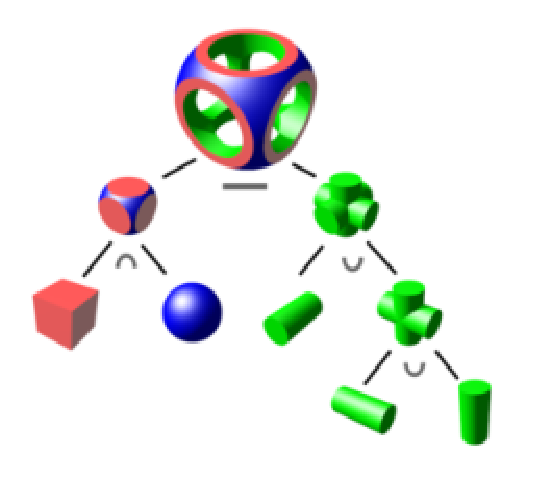
\includegraphics{csg_ex.eps}
  \caption{An example of how CSG volumes are created using Boolean combinations
    of smaller objects. The union of the three orthogonal cylinders is
    subtracted from the intersection of the box and sphere on the left to form
    the final volume at the top of the figure.}
  \label{fig:csg_ex}
\end{figure}

It is possible to construct complex geometries using CSG, but, as mentioned in
the introduction, the interface for this work is typically text-based and
defining complex volumes is a tedious and time-consuming task. Detecting
problems with the geometry definition is straightforward for the same reason
that particles can be robustly tracked through the geometry - the analytic
description of the surfaces. Fixing undefined regions of the geometry or
detecting invalid volume definitions is more difficult however.

The detection of intersections and particle containment queries in CSG
geometries is in practice computationally inexpensive for relatively simple
volume definitions, but due to the logical combinations of surfaces used to
create volumes the number of evaluations necessary to satisfy these queries is
linear with the number of surfaces in the definition. For sufficiently large and
complex models, it is not uncommon for volumes with many surfaces to be
artificially separated by planes to create two volumes with fewer surfaces in
their definition.

Visualization of CSG models can also be difficult. Because native formats for
CSG differ greatly between each Monte Carlo code, each typically comes with its
own visualization tools. These tools are typically restricted to 2D images of
the model representing a user-specified slice through the geometry. Other tools
such as MCAM \cite{Liu_2005} and McCad \cite{Tsigetamirat_2008} allow for
interactive visualization and repair of CSG models they do not provide the
accuracy of CAD modeling engines.

\subsection{CAD Geometry}

CAD systems allow for highly efficient and accurate geometric
representation. Highly complex models can be created using interactive
visualization tools represented in 3D space with a rich tool set for volume and
surface creation. These tools and the immediate visual verification of a user's
work reduces human error in model generation and design iteration.

In addition to reducing human error, CAD models provide a common domain for
analysis in other engineering domains such as fluid dynamics, heat transfer,
and structural engineering. This shared domain creates a common domain for
coupled physics simulation.

CAD also has the ability to represent free-form or higher-order surface. The use
of representations like splines and subdivision surfaces allow for more accurate
representation.

\subsection{Monte Carlo Radiation Transport on CAD Geometry}

The Direct Accelerated Geometry Monte Carlo (DAGMC) toolkit is a software
capable of Monte Carlo radiation transport directly on CAD models
\cite{Tautges_2009}. DAGMC was developed at the University of Wisconsin -
Madison. It has been coupled with many Monte Carlo codes to enable analysis on
CAD models. DAGMC relies on Cubit (and its commercial counterpart, Trelis) for CAD
modeling. Both of these CAD packages rely on the geometric modeling kernel,
ACIS.

DAGMC provides robust particle tracking for Monte Carlo transport on
arbitrarily complex CAD geometries. It accomplishes this by discretizing CAD
surfaces into sets of triangles. Volumes are then defined by any triangles which
represent bounding surfaces of a given volume. This surface mesh and the
geometric relationships between the mesh entities are stored in the Mesh
Oriented dAtaBase (MOAB) \cite{Tautges_2004}. These relationships are stored in
a hierarchical structure within MOAB, relating volumes to their surfaces,
surfaces to curves, and curves to vertices. 

It is important that geometric relationships of the mesh are maintained to
accelerate certain geometric queries on the surface mesh. For example,
\textit{Next Volume} queries are accelerated by using these relationships to
directly determine which volume a particle is passing into upon crossing a
surface rather than performing a query of the particle's location for each
volume. Other queries become more complicated due to the sheer number of
triangles needed to properly define volumes with detailed features. 

Next surface and closest to location geometry queries, for example, can be very
computationally expensive for volumes composed of hundreds of thousands or even
millions of triangles. A convenient way to think about performing geometric queries on
triangulated surfaces or volumes is to consider an equivalent CSG representation
constructed using a series of intersecting planes in place of triangles. The
structure imposed by the Boolean combinations used to define such volumes
require that each surface be checked for an intersection with the particle
trajectory. The nearest of these intersections can then be used to determine a
particle's crossing or movement to the physics event location specified by the
attached Monte Carlo code.

The problem of finding in intersection of a given particle location and
trajectory with a set of geometric primitives is known as ray tracing and is
well-studied in the field of computer graphics and animation. In this field,
data structures designed to accelerate the location of the nearest ray
intersection are applied.

\section{Ray Tracing Acceleration Data Structures}

Acceleration data structures for ray tracing are designed to rapidly narrow the
search for an intersection in virtual space given a starting position and
direction also known as a ray. This is accomplished by partitioning the space
and associating geometric primitives, most commonly triangles, with that
bounding partition. A search is performed by checking for an intersection with
the bounding partition. If the ray does not intersect with the partition, then
the set of primitives associated with that partition can be removed from the
search. If the ray does intersect with the partition, then the set of associated
primitives must be checked for intersection. Because a single separation into
two spatial partitions is often not enough to increase search efficiency, this
partitioning process is performed recursively. The result is a tree structure in
which at the top of the tree partitions are associated other partitions, known
as child nodes, rather than primitives. At the bottom of the tree exists a set of
nodes called leaves which are associated with geometric primitives. 

The search for a ray intersection then becomes a traversal of the tree
in which the children of the root node are checked for intersection. If an
intersection is found with one or both of the nodes, then the corresponding child nodes 
are checked for intersection as well. This process is repeated until leaf nodes
are reached at which point primitives are checked for intersection. Knowing that
a ray which doesn't intersect with a bounding partition cannot intersect with
any of the primitives it contains, allows many primitives to be rapidly removed
from the search and the number of intersection checks with primitives limited to
a small few. This technique reduces the algorithmic complexity of the search
from a brute force, or linear, $O(log(N_{triangles})$ to an $O(\,
log(N_{primitives}))$ search. 

\subsection{Partition Splitting Heuristics}

There are two components that go into the creation of spatial
partitions. The first is the selection of a candidate splitting plane which is
used to separate entities into one partition or another. The second is
the evaluation of the ``cost'' of that split should it be used. This cost is an
estimate of how good or bad the split would be. Because there is no way to know
exactly how expensive or inexpensive a split will be for the particular
simulation at hand, heuristics are used to evaluate this cost and determine the
optimal splitting plane using limited information about the local tree. This
information is typically limited to the number of primitives and bounds of the
parent partition and resulting child partitions.

The two heuristics will be addressed here - the Entity Ratio Heuristic (ERH) and the
Surface Area Heuristic (SAH). The ERH uses only the resulting number of
primitives in each child node to determine the cost of a split. The philosophy
behind this heuristic is to maintain the expected $O(log(N_{triangles})$ cost of
a ray traversal by ensuring that primitives are split as evenly as possible from
parent to child node. A form of this heuristic is presented in
Eq. \ref{eq:ERH}. This heuristic is unitless and bounded by zero and
one. This makes is possible to set both an upper and lower bound on the
unacceptable cost and a ``good enough'' cost.

\begin{figure}[H]
\begin{equation}
\label{eq:ERH}
 C = \frac{|P_{R}-P_{L}|}{(P_{R} + P_{L})} 
\end{equation}
  \begin{align*}
    C - & \,final \, cost \, evaluation \\
    P_{L} - & \, primitives\, contained\, by\, the\, left\, child  \\
    P_{R} - & \, primitives\, contained\, by\, the\, right\, child \\
  \end{align*}
  \caption{An example of the entity ratio calcution for a binary tree.}
  \label{fig:ERH}
\end{figure}

The SAH applies spatial information as well as division of primitives to the
cost evaluation. The SAH uses the surface area of candidate child partitions
relative to the current partition's surface area as an approximation for the
probability that the child will be visited after the parent volume. The explicit
form of the surface area heuristic was introduced in 1987 by Goldsmith and
Salmon \cite{Goldsmith_1987} and later formalized by MacDonald and Booth in 1990
\cite{MacDonald_1990}. Its full form is found in Equation \ref{eq:SAH}.

\begin{figure}[H]
  \begin{equation}
    C =  C_{t} + \frac{SA_{L}}{SA_{P}} |P_{L}|C_{i} +  \frac{SA_{R}}{SA_{P}} |P_{R}|C_{i}
    \label{eq:SAH}
  \end{equation}
  \begin{align*}
    C_{t} - & \,cost\, of\, traversal\, to\, child\, nodes \\
    C_{i} - & \, cost\, of\, primitive\, intersection\, check\, \\
    SA_{L} - &  \,surface\, area\, of\, left\, child \\
    P_{L} - & \, primitives\, contained\, by\, the\, left\, child  \\
    SA_{R} - & \, surface\, area\, of\, right\, child \\
    P_{R} - & \, primitives\, contained\, by\, the\, right\, child \\
    SA_{P} - & \, parent\, bounding\, volume \\
  \end{align*}
  \caption{A form of the surface area heuristic for a binary tree.}
  \label{fig:SAH}
\end{figure}

For the general case, ERH has not proved to be as effective as the SAH, but it
has proven to be a useful tool in correcting the surface area heuristic for
triangle mesh features of a specific type. This scenario will be discuss further
in <INSERT HV CHAPTER HERE>.

% 
\section{Motivation}

\begin{frame}
  \frametitle{CAD-Based Monte Carlo}
\end{frame}

% \include{related/related}

%% etc, etc.

%% Do you have appendices?  If so, add them here, just like chapters.
% \begin{appendices}
% \include{backmatter/appendix1}
% \end{appendices}

%% Are you a big nerd with a colophon?  Add it here.
\begin{colophon}
\svnidlong{$LastChangedBy$}{$LastChangedRevision$}{$LastChangedDate$}{$HeadURL: http://freevariable.com/dissertation/trunk/frontmatter.tex $}
\vcinfo{}

This template uses Gyre Pagella by default.  (I used Arno Pro in my dissertation.)

Feel free to give me a shout-out in your colophon or acks if this template is useful for you.  Good luck!

\end{colophon}

%% McBride is a very nice style (some version is included in this distribution)
\bibliographystyle{mcbride}
\bibliography{refs}

%% Want an index?  Neither did I.
%\printindex

\end{document}
